\documentclass[12pt,a4paper]{article}
\usepackage{ctex}
\usepackage{geometry}
\usepackage{graphicx}
\usepackage{setspace}
\usepackage{listings}
\usepackage{listingsutf8}
\usepackage{xcolor}
\usepackage{hyperref}
\usepackage{float} 


\geometry{left=3cm,right=3cm,top=2.5cm,bottom=2.5cm}

% 代码样式
\lstset{
    language=Java,
    inputencoding=utf8,
    basicstyle=\ttfamily\small,
    keywordstyle=\color{blue}\bfseries,
    commentstyle=\color{green!50!black},
    stringstyle=\color{orange},
    showstringspaces=false,
    numbers=left,
    numberstyle=\tiny,
    breaklines=true,
    frame=single
}

\begin{document}

% ================= 封面 =================
\begin{titlepage}
\centering

% 校徽 Logo 
\makebox[\textwidth][c]{%
  
\includegraphics[height=4cm]{fengmian.png}%
}
\vspace*{2cm}

% 学院名称
{\zihao{1}\heiti 信息科学与工程学院}\\[1cm]

% 学年学期
{\zihao{4} 2025---2026 \kaishu学年第一学期}\\[1.5cm]

% 报告标题
\makebox[\textwidth][c]{%
  
\includegraphics[height=2cm]{shiyanbaogao.png}%
}
\\[2em] % 空行
% 实验基本信息表
\zihao{4} 
\renewcommand{\arraystretch}{1.8} % 表格行距
\begin{tabular}{rl}
\heiti 课程名称: & \underline{\makebox[18em][c]{\fangsong Java 编程技术}} \\
\vspace{1cm}
\heiti 实验名称: & \underline{\makebox[18em][c]{\fangsong 一个简单的控制台应用程序}} \\
\kaishu 专  业  班  级 & \underline{\makebox[18em][c]{\kaishu 通信一班}} \\
\kaishu 学  生  学  号 & \underline{\makebox[18em][c]{\kaishu 202300120317}} \\
\kaishu 学  生  姓  名 & \underline{\makebox[18em][c]{\kaishu 陈都阳}} \\
\kaishu 实  验  时  间 & \underline{\makebox[18em][c]{\kaishu 2025年9月16日}} \\
\end{tabular}

\vfill
\end{titlepage}

% ================= 正文 =================
\section*{【实验目的】}
\begin{enumerate}
    \item 熟悉Java Applet的开发。
    \item 学会Java的swing组件。
\end{enumerate}

\section*{【实验要求】}
\begin{enumerate}
    \item 编写一个简单的Java Applet程序,该程序输出两行文字:\\
    “这是一个Java Applet程序” 和 “我改变了字体”。
    \item 按要求完成实验一到实验五。
    \item 编译运行,并截图实验结果。
    \item 实验后回答相关思考问题。
\end{enumerate}

\section*{【第一个实验具体内容】}

\subsection*{源代码}
\begin{figure}[H]
\centering
\begin{lstlisting}
// MyFirstApplet.java
package TwoJavaExam;
import java.applet.Applet;
import java.awt.Color;
import java.awt.Font;
import java.awt.Graphics;

public class MyFirstApplet extends Applet {
    @Override
    public void paint(Graphics g) {
        g.setColor(Color.blue);
        g.setFont(new Font("Serif", Font.BOLD, 28));
        g.drawString("Hello, this is my first Applet!", 20, 50);

        g.setColor(Color.red);
        g.setFont(new Font("SansSerif", Font.BOLD, 36));
        g.drawString("Java Applet Demo", 20, 100);
    }
}

\end{lstlisting}
\caption{MyFirstApplet 源代码}
\end{figure}

\subsection*{实验过程与结果}

\begin{figure}[H]
\centering
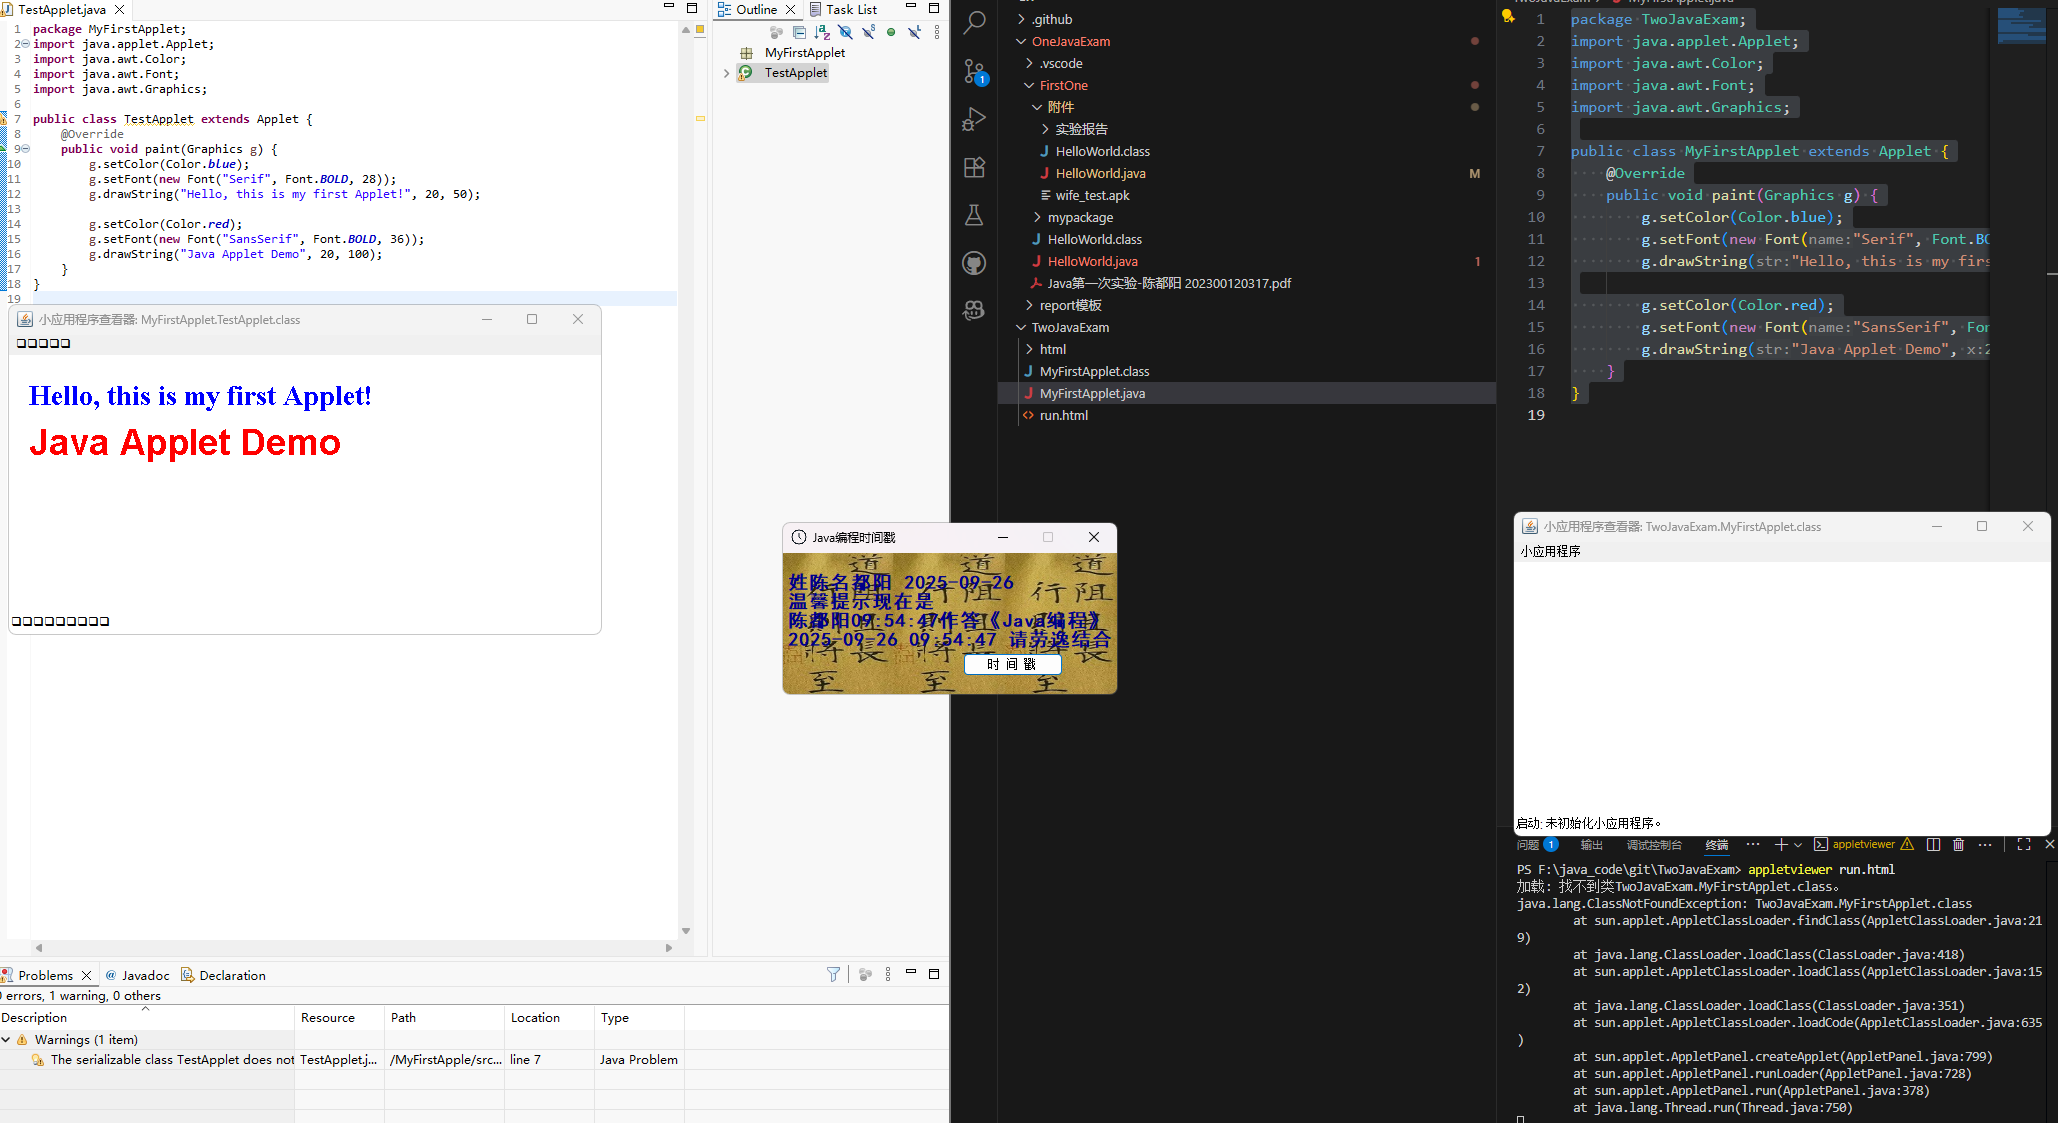
\includegraphics[width=0.8\textwidth]{one.png}
\caption{运行结果}
\end{figure}


\section*{思考与分析}
\begin{enumerate}
    \item 主类不用 public 修饰,通常可以编译通过(是可编译的):主类如果不使用 public,它是 package-private(默认访问权限),javac 可以正常编译该类。
    \item 主类不用 public 修饰,程序通常也能运行(JVM 可启动包内默认访问的类):JVM 加载类时并不要求该类为 public,只要你使用正确的类名(包括包名),java 命令可以启动包含 public static void main(String[]) 的 package-private 类。
    \item 把 paint 写成 Paint:如果没有重写注解,源代码会编译通过(因为这是一个新方法):从Applet里面扒拉的方法没用,你自己写的方法名也不与框架中的方法名冲突。
    \item 把 paint 写成 Paint:运行时不会被 AWT/Applet 框架调用,因此看不到你的绘制输出(除非你手动调用该方法)。自己重写的方法在Applet里面没被调运,运行原来的paint函数。
    \item 还有一个问题,在vscode里面编写的html文件不能启动第一个问题的代码,但是更改路径启动其他Java文件却完全可以。
\end{enumerate}

\section*{【第二个实验具体内容】}

\subsection*{源代码}
\begin{figure}[H]
\centering
\begin{lstlisting}
// TwoQuestion.java
package TwoJavaExam;

public class TwoQuestion {
    private int start;
    private int end;
    public TwoQuestion(int start, int end) {
        this.start = start;
        this.end = end;
    }
    public boolean IsPrime(int n) {
        if (n < 2) return false;
        for (int i = 2; i <= Math.sqrt(n); i++) {
            if (n % i == 0) return false;
        }
        return true;
    }
    public int SumPrimes() {
        int sum = 0;
        for (int i = start; i <= end; i++) {
            if (IsPrime(i)) {
                sum += i;
            }
        }
        return sum;
    }
    public static void main(String[] args) {
    TwoQuestion pc = new TwoQuestion(1, 1000);
    int sum = pc.SumPrimes();
    System.out.println("Sum of primes from 1 to 1000: " + sum);
    }
}


\end{lstlisting}
\caption{TwoQuestion 源代码}
\end{figure}

\subsection*{实验过程与结果}

\begin{figure}[H]
\centering
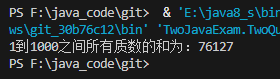
\includegraphics[width=0.8\textwidth]{two.png}
\caption{运行结果}
\end{figure}

\section*{【第三个实验具体内容】}

\subsection*{源代码}
\begin{figure}[H]
\centering
\begin{lstlisting}
// ThreeQusetion.java
package TwoJavaExam;

public class ThreeQusetion {
	private int start;
	private int end;

	public ThreeQusetion(int start, int end) {
		this.start = start;
		this.end = end;
	}

	public int Factorial(int n) {
		if (n <= 1) return 1;
		return n * Factorial(n - 1);
	}

	public int SumFactorials() {
		int sum = 0;
		for (int i = start; i <= end; i++) {
			sum += Factorial(i);
		}
		return sum;
	}

	public static void main(String[] args) {
		ThreeQusetion tq = new ThreeQusetion(1, 10);
		int sum = tq.SumFactorials();
		System.out.println("1! + 2! + ... + 10! =" + sum);
	}
}



\end{lstlisting}
\caption{ThreeQuestion 源代码}
\end{figure}

\subsection*{实验过程与结果}

\begin{figure}[H]
\centering
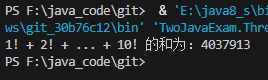
\includegraphics[width=0.8\textwidth]{three.png}
\caption{运行结果}
\end{figure}

\section*{【第四个实验具体内容】}
\subsection*{流程图}

\begin{figure}[H]
\centering
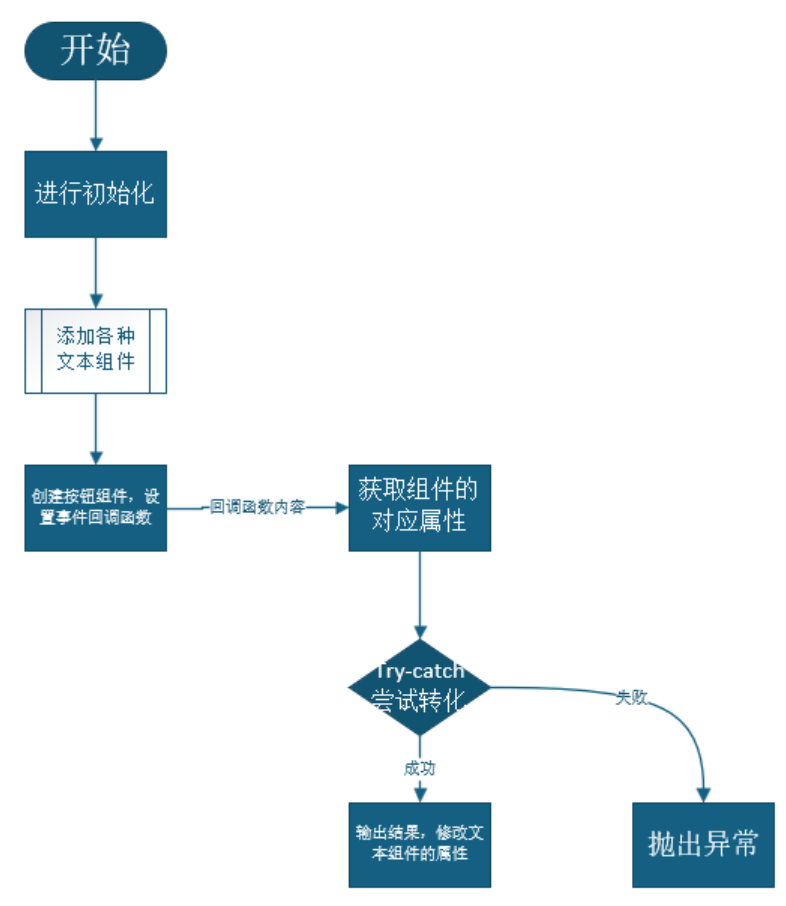
\includegraphics[width=0.8\textwidth]{four1.png}
\caption{流程图}
\end{figure}

\subsection*{源代码}
\begin{figure}[H]
\centering
\begin{lstlisting}
// FourQusetion.java
package TwoJavaExam;

import java.applet.Applet;
import java.awt.*;
import java.awt.event.*;

public class FourQuestionSimple extends Applet implements ActionListener {
    private TextField inputField;
    private Choice typeChoice;
    private Label resultLabel;
    private Button convertButton;
    private TextArea historyArea;
    private String historyText = ""; 

    public void init() {
        setLayout(new FlowLayout());
        add(new Label("Enter temperature:"));
        inputField = new TextField(10);
        add(inputField);

        typeChoice = new Choice();
        typeChoice.add("Celsius to Fahrenheit");
        typeChoice.add("Fahrenheit to Celsius");
        add(typeChoice);

        convertButton = new Button("Convert");
        convertButton.addActionListener(this);
        add(convertButton);

        resultLabel = new Label("Result will be displayed here");
        add(resultLabel);

        add(new Label("History:"));
        historyArea = new TextArea(5, 30);
        historyArea.setEditable(false);
        add(historyArea);
    }
\end{lstlisting}
\end{figure}
\begin{figure}[H]
\centering
接上页代码
\begin{lstlisting}
    public void actionPerformed(ActionEvent e) {
        String input = inputField.getText().trim();
        if (input.equals("")) {
            resultLabel.setText("Please enter a temperature value!");
            return;
        }

        try {
            double value = Double.parseDouble(input);
            double resultValue;
            String result;

            if (typeChoice.getSelectedIndex() == 0) {
                resultValue = value * 9 / 5 + 32;
                result = value + " Celsius = " + String.format("%.2f", resultValue) + " Fahrenheit";
            } else {
                resultValue = (value - 32) * 5 / 9;
                result = value + " Fahrenheit = " + String.format("%.2f", resultValue) + " Celsius";
            }

            resultLabel.setText(result);
            historyText += result + "\n";
            historyArea.setText(historyText);

        } catch (NumberFormatException ex) {
            resultLabel.setText("Invalid input! Please enter a valid number.");
        }
    }
}
\end{lstlisting}

\caption{FourQuestion 源代码}
\end{figure}

\subsection*{实验过程与结果}

\begin{figure}[H]
\centering
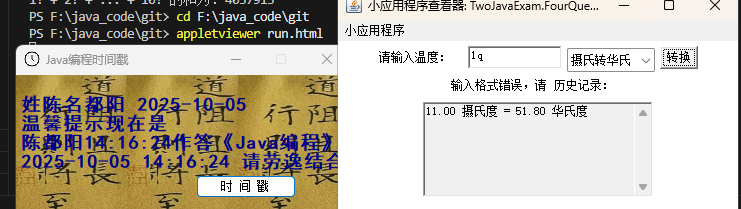
\includegraphics[width=0.8\textwidth]{four.png}
\caption{运行结果}
\end{figure}

\section*{【第五个实验具体内容】}
\subsection*{流程图}

\begin{figure}[H]
\centering
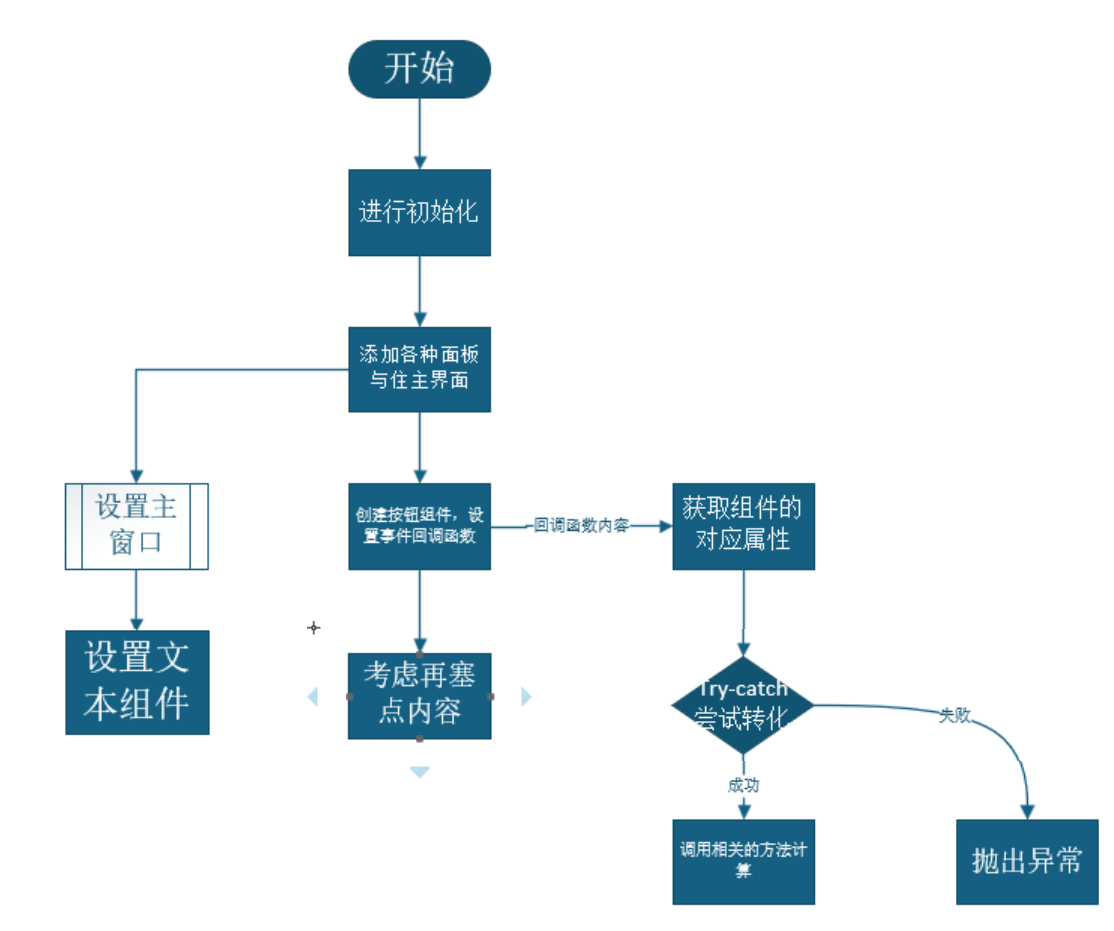
\includegraphics[width=0.8\textwidth]{five1.png}
\caption{流程图}
\end{figure}

\subsection*{源代码}
\begin{figure}[H]
\centering
\begin{lstlisting}
// FiveQusetion.java
package TwoJavaExam;

import javax.swing.*;
import java.awt.*;
import java.io.*;
import java.nio.charset.StandardCharsets;
import java.nio.file.Files;
import java.text.DecimalFormat;
import java.util.HashMap;
import java.util.Map;

public class FiveQuestion {

    // User database
    private Map<String, String> userDatabase = new HashMap<>();

    // GUI components
    private JFrame mainFrame;
    private JTextField usernameField;
    private JPasswordField passwordField;
    private JTextField electricityUsageField;
    private JLabel resultLabel;
    private DecimalFormat decimalFormat = new DecimalFormat("0.00");

    // Constructor
    public FiveQuestion() {
        // Default anonymous user
        userDatabase.put("anonymous", "anonymous");
        CreateAndShowGUI();
    }
\end{lstlisting}
\end{figure}
\begin{figure}[H]
接上页代码
\begin{lstlisting}
    private void CreateAndShowGUI() {
        mainFrame = new JFrame("Tiered Electricity Bill Calculator");
        mainFrame.setDefaultCloseOperation(JFrame.EXIT_ON_CLOSE);
        mainFrame.setSize(420, 300);
        mainFrame.setLocationRelativeTo(null);
        JTabbedPane tabbedPane = new JTabbedPane();
        tabbedPane.addTab("Login", BuildLoginPanel());
        tabbedPane.addTab("Bill Calculation", BuildCalculationPanel());
        tabbedPane.addTab("User Management", BuildUserManagementPanel());

        mainFrame.getContentPane().add(tabbedPane);
        mainFrame.setVisible(true);
    }

    // Login panel
    private JPanel BuildLoginPanel() {
        JPanel panel = new JPanel(new GridBagLayout());
        GridBagConstraints gbc = new GridBagConstraints();
        gbc.insets = new Insets(6, 6, 6, 6);

        gbc.gridx = 0; gbc.gridy = 0;
        panel.add(new JLabel("Username:"), gbc);

        gbc.gridx = 1;
        usernameField = new JTextField(12);
        panel.add(usernameField, gbc);

        gbc.gridx = 0; gbc.gridy = 1;
        panel.add(new JLabel("Password:"), gbc);
\end{lstlisting}
\end{figure}
\begin{figure}[H]
接上页代码
\begin{lstlisting}
        gbc.gridx = 1;
        passwordField = new JPasswordField(12);
        panel.add(passwordField, gbc);

        JButton loginButton = new JButton("Login");
        loginButton.addActionListener(e -> HandleLogin());
        gbc.gridx = 0; gbc.gridy = 2; gbc.gridwidth = 2;
        panel.add(loginButton, gbc);

        return panel;
    }

    // Calculation panel
    private JPanel BuildCalculationPanel() {
        JPanel panel = new JPanel(new GridBagLayout());
        GridBagConstraints gbc = new GridBagConstraints();
        gbc.insets = new Insets(6, 6, 6, 6);

        gbc.gridx = 0; gbc.gridy = 0;
        panel.add(new JLabel("Enter electricity usage (kWh):"), gbc);

        gbc.gridx = 1;
        electricityUsageField = new JTextField(10);
        panel.add(electricityUsageField, gbc);

        JButton calculateButton = new JButton("Calculate Bill");
        calculateButton.addActionListener(e -> HandleCalculation());
        gbc.gridx = 0; gbc.gridy = 1; gbc.gridwidth = 2;
        panel.add(calculateButton, gbc);

        resultLabel = new JLabel("Result:");
        gbc.gridy = 2;
        panel.add(resultLabel, gbc);

        return panel;
    }
\end{lstlisting}
\end{figure}
\begin{figure}[H]
接上页代码
\begin{lstlisting}
    // User management panel
    private JPanel BuildUserManagementPanel() {
        JPanel panel = new JPanel(new BorderLayout());
        JPanel topPanel = new JPanel();

        JButton importButton = new JButton("Import Users from TXT");
        JButton exportButton = new JButton("Export Users to TXT");

        importButton.addActionListener(e -> ImportUsers());
        exportButton.addActionListener(e -> ExportUsers());

        topPanel.add(importButton);
        topPanel.add(exportButton);
        panel.add(topPanel, BorderLayout.NORTH);

        JTextArea infoArea = new JTextArea(8, 30);
        infoArea.setEditable(false);
        UpdateUserInfo(infoArea);

        panel.add(new JScrollPane(infoArea), BorderLayout.CENTER);
        panel.putClientProperty("infoArea", infoArea);
        return panel;
    }

    private void UpdateUserInfo(JTextArea infoArea) {
        StringBuilder sb = new StringBuilder("Current user list:\n");
        for (String username : userDatabase.keySet()) {
            sb.append(username).append("\n");
        }
        infoArea.setText(sb.toString());
    }
\end{lstlisting}
\end{figure}
\begin{figure}[H]
接上页代码
\begin{lstlisting}
    // Login logic
    private void HandleLogin() {
        String username = usernameField.getText().trim();
        String password = new String(passwordField.getPassword());

        if (username.isEmpty()) {
            JOptionPane.showMessageDialog(mainFrame, "Username cannot be empty", "Error", JOptionPane.ERROR_MESSAGE);
            return;
        }

        String storedPassword = userDatabase.get(username);
        if (storedPassword != null && storedPassword.equals(password)) {
            JOptionPane.showMessageDialog(mainFrame, "Login successful", "Info", JOptionPane.INFORMATION_MESSAGE);
        } else {
            JOptionPane.showMessageDialog(mainFrame, "Invalid username or password", "Error", JOptionPane.ERROR_MESSAGE);
        }
    }

    // Bill calculation logic
    private void HandleCalculation() {
        String input = electricityUsageField.getText().trim();
        if (input.isEmpty()) {
            JOptionPane.showMessageDialog(mainFrame, "Please enter electricity usage", "Error", JOptionPane.ERROR_MESSAGE);
            return;
        }
\end{lstlisting}
\end{figure}
\begin{figure}[H]
接上页代码
\begin{lstlisting}
        try {
            double usage = Double.parseDouble(input);
            if (usage < 0) throw new NumberFormatException();

            double cost = CalculateTieredCost(usage);
            resultLabel.setText("Result: " + decimalFormat.format(cost) + " yuan");
        } catch (NumberFormatException ex) {
            JOptionPane.showMessageDialog(mainFrame, "Please enter a valid non-negative number", "Error", JOptionPane.ERROR_MESSAGE);
        }
    }

    // Tiered billing calculation
    private double CalculateTieredCost(double usage) {
        double cost;
        if (usage <= 240) {
            cost = usage * 0.55;
        } else if (usage <= 540) {
            cost = 240 * 0.55 + (usage - 240) * 0.70;
        } else {
            cost = 240 * 0.55 + (540 - 240) * 0.70 + (usage - 540) * 0.95;
        }
        return cost;
    }

    // Import users from TXT
    private void ImportUsers() {
        JFileChooser fileChooser = new JFileChooser();
        int result = fileChooser.showOpenDialog(mainFrame);
        if (result == JFileChooser.APPROVE_OPTION) {
            File file = fileChooser.getSelectedFile();
\end{lstlisting}
\end{figure}
\begin{figure}[H]
接上页代码
\begin{lstlisting}
            try {
                for (String line : Files.readAllLines(file.toPath(), StandardCharsets.UTF_8)) {
                    String trimmed = line.trim();
                    if (trimmed.isEmpty()) continue;
                    String[] parts = trimmed.split(",");
                    if (parts.length >= 2) {
                        userDatabase.put(parts[0].trim(), parts[1].trim());
                    }
                }
                JOptionPane.showMessageDialog(mainFrame, "Import completed", "Info", JOptionPane.INFORMATION_MESSAGE);
                RefreshUserPanel();
            } catch (IOException ex) {
                JOptionPane.showMessageDialog(mainFrame, "Import failed: " + ex.getMessage(), "Error", JOptionPane.ERROR_MESSAGE);
            }
        }
    }

    // Export users to TXT
    private void ExportUsers() {
        JFileChooser fileChooser = new JFileChooser();
        int result = fileChooser.showSaveDialog(mainFrame);
        if (result == JFileChooser.APPROVE_OPTION) {
            File file = fileChooser.getSelectedFile();
            try (BufferedWriter writer = Files.newBufferedWriter(file.toPath(), StandardCharsets.UTF_8)) {
                for (Map.Entry<String, String> entry : userDatabase.entrySet()) {
                    writer.write(entry.getKey() + "," + entry.getValue());
                    writer.newLine();
                }
                JOptionPane.showMessageDialog(mainFrame, "Export completed", "Info", JOptionPane.INFORMATION_MESSAGE);
            } 
\end{lstlisting}
\end{figure}
\begin{figure}[H]
接上页代码
\begin{lstlisting}
            catch (IOException ex) {
                JOptionPane.showMessageDialog(mainFrame, "Export failed: " + ex.getMessage(), "Error", JOptionPane.ERROR_MESSAGE);
            }
        }
    }

    // Refresh user panel
    private void RefreshUserPanel() {
        Window[] windows = Window.getWindows();
        for (Window window : windows) {
            if (window instanceof JFrame) {
                JFrame frame = (JFrame) window;
                for (Component component : frame.getContentPane().getComponents()) {
                    if (component instanceof JTabbedPane) {
                        JTabbedPane tabbedPane = (JTabbedPane) component;
                        for (int i = 0; i < tabbedPane.getTabCount(); i++) {
                            Component comp = tabbedPane.getComponentAt(i);
                            if (comp instanceof JPanel) {
                                JPanel panel = (JPanel) comp;
                                JTextArea infoArea = (JTextArea) panel.getClientProperty("infoArea");
                                if (infoArea != null) UpdateUserInfo(infoArea);
                            }
                        }
                    }
                }
            }
        }
    }
\end{lstlisting}
\end{figure}
\begin{figure}[H]
接上页代码
\begin{lstlisting}
    public static void main(String[] args) {
        new FiveQuestion();
    }
}

\end{lstlisting}

\caption{FiveQuestion 源代码}
\end{figure}

\subsection*{实验过程与结果}

\begin{figure}[H]
\centering
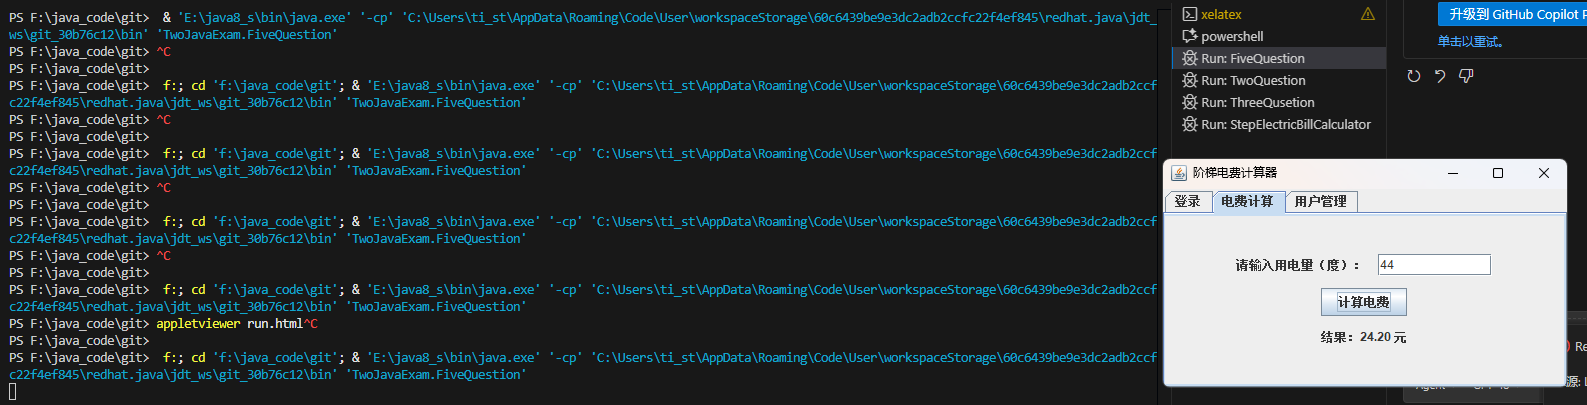
\includegraphics[width=0.8\textwidth]{five.png}
\caption{运行结果}
\end{figure}

\section*{【实验心得】}
    本次实验主要花费时间在applet的运行上,由于使用的idea不支持applet的运行,所以花费了较多时间在环境配置上,最终使用vscode成功运行。早期想通过虚拟机安装IE6来运行applet,但是由于虚拟机的性能问题,塞不进去java8,最终放弃。
后面通过查询找到了一个较为可行的解决发案,使用appletviewer来运行applet程序,成功解决问题。但是第一个简单的代码却无法运行,包和路径都没问题,也没有中文,但是就是无法运行。

    还有针对第四个和第五个实验,我做了一些修正,就第四个而言,都上UI界面了,那得对用户友好一些,我加入了历史记录查询,应为是手输的代码,包有一些写错的,这时候历史记录可以快速的查询,后续可以加一些功能,将文本组件的数值属性保存到excel表格中,每天定时把数据通过邮箱,局域网共享给负责审核的人,确保数据正确,也可以塞入一个回调函数,实现表格数据转化,不过这个功能matlab更好一些,excel的宏指令也能实现,意义不是很大。

    第五个实验,我做了一些修改,增加了用户管理功能,由于数据都是通过txt文件保存的,后续可以直接用爬虫从对应的电费网站上扒拉用户的电费情况,导入数据后通过分析,每月定时通过邮件或者局域网发给对应的用户,实现账单推送。可能是我太菜了,java的GUI用起来不如C\#的窗体程序好用。要是当年C\#在Java占据市场前出现,微软也不会不管C\#的。在c\#很好调用其他类型文件的
,要是利用vbs文件直接操控电脑,比如电费超额,1s后直接调用vbs脚本来关机,或者电费的属性改为积分制来管小孩上网也行。

\end{document}
